% This file is iccc.tex.  It contains the formatting instructions for and acts as a template for submissions to ICCC.  It borrows liberally from the AAAI and IJCAI formats and instructions.  It uses the files iccc.sty, iccc.bst and iccc.bib, the first two of which also borrow liberally from the same sources.

\documentclass[letterpaper]{article}
\usepackage{iccc}

\usepackage{graphicx}
\usepackage{times}
\usepackage{helvet}
\usepackage{courier}
\pdfinfo{
	/Title (Anything2vec: generalizing word2vec via the use of meaningful contexts)
	/Subject (Proceedings of ICCC)
	/Author (ICCC)}
% The file iccc.sty is the style file for ICCC proceedings.
%

%\title{Anything2vec: generalizing word2vec via the use of meaningful
%	contexts}
% Add something about its application to trope description - JJ 
%\author{Dan Ventura\\
%Computer Science Department\\
%Brigham Young University\\
%Provo, UT 84602  USA\\
%ventura@cs.byu.edu\\
%}
\setcounter{secnumdepth}{0}

\begin{document} 
	% \maketitle
	\begin{abstract}
		\begin{quote}
			% From the old paper:
			%   Word2vec has been a very successful algorithm that is able to give a
			% semantic representation to words on a corpus based in the context
			% they appear. In this paper we will try to extend this concept to
			% other {\em unordered} contexts. We will try to define this context
			% for movie (and TV) tropes.
			In this paper we present a generalized approach to extend the use of word2vec for non traditional NLP (Natural Language Processing). In order to exemplify the idea we use tvtropes dataset (trope names and film names only) to create a text corupus in order to give contextual information to any pice of data.
		\end{quote}
	\end{abstract}
	
	% From the old paper:
	% What are tropes and why we are interested
	
	% We need to find an embedding for tropes that allows us to do trope arithmetic and also process them, and movies in which they are used, in an uniform way.
	
	% We propose trope2vec
	
	% We analyze how it allows to explore the trope space and find
	% similarities between them.
	
	\section{Introduction}
	
	% Motivation: we need to have a representation that is
	% * That includes the context of the trope
	% * relatively compact
	% * capable of doing arithmetic
	% * uniform for tropes and movies.
	
	This work aims to find a knowledge representation and a new methodology to apply machine learning techniques to entities without a natural language context. To exemplify this new methodology, tropes and films from tvtropes.org are used. That representation and methodology will let us, for example, to discover wich set of tropes will be affordable to create a new block buster film or a new best seller book.   \\
	
	Tv Tropes (tvtropes.org) is a collaborative website created in 2004 to share information about tips, narrative or cinematographic techniques used in creative works such as movies, tv series, advertaising, videogames, sports, comics or books. Tvtropes.org defines tropes as: "a storytelling device or convention, a shortcut for describing situations the storyteller can reasonably assume the audience will recognize." Articles to describe tropes are writed usually with a very expresive and non formal vocabulary. Each film, tv serie or other fiction element usually include a description and a list of asociated tropes. Tropes pages usually contains a description followed by a list of films or a narrative resource that uses this trope.\\
	
	To represent tropes we decided to use embeedings vectors foç r each trope. This representation should allow us to perform concept arithmetic. This property will be very interesting since our goal is to determine, for example, which group of tropes must have a successful film. Applying arithmetic of concepts about tropes we could, for example, find classic western movies, which have their main narrative characteristics, but the western one is replaced by space adventure trope. in order to obtain the set of embeeding vects associated with the tropes we will use word2vec \cite{mikolov2013}. Since the development of this technique in 2013 word2vec is one of the techniques for the generation of embeeding vectors from natural language (NLP) most used. However word2vec has not only been used to obtain embeeding vectors of texts in natural language. Other works like \cite{kazama2018} have shown that it is possible to use word2vec to obtain vectors from non-NLP information sources. Our approach is based on the use of the fundamental elements of information (in our case the tropes) to generate an artificial narrative or corpus that can give a similar meaning to the concepts that they would have in a text written by humans. This artificially created text should represent the relationships between entities in the same way that a human would relate them in a descriptive text about these entities. If the artificial corpus is correctly constructed, it should produce some embeeding vectors with the capacity to offer us a correct arithmetic of concepts. \\
	
	% How we want to solve that problem: we think that an adaptation of word2vec should be possible
	
	% One of the most important elements in NLP (Natural Language Processing) is the context where words appear inside a text. One of the most popular algorithms to associte numerical vectors to words is word2vec \cite{mikolov2013}. This algorithm use words that are before and after a target word in order to contextualize words. But, what happend if we don't have a text to start analyzing words? What happend if we only have relationships between terms like this trope appear in this film? For this type of problem we purpouse a generalization in the use of word2vec algorithm that let to build a context for related terms. 
	
	% (Talk about A Neural Network System for Transformation of Regional Cuisine Style \cite{kazama2018} and other non-NLP word2vec use like E-commerce in Your Inbox: Product Recommendations at Scale \cite{Grbovic2015} or Meta-Prod2Vec - Product Embeddings Using Side-Information for Recommendation \cite{vasile2016}
	
	% How we do it:
	% * Methodology for creating the context of every trope
	% * Methdology for representing movies using trope vector
	% * How we evaluate the goodness of the set of movies/tropes chosen.
	
	% Our results
	% * Clustering
	% * Graph representation
	% * Movie representation
	% * Example of synthetic movie generation.
	
The rest of the paper is organized as follows. Next we present the
state of the art in using embeddings for problems other than language
processing, as well as an overview of the use of tropes for narrative
generation. The methodology is presented next in Section
\ref{sec:met}, with results presented in Section \ref{sec:res}
followed by the conclusion that closes the paper.

        
\section{State of the art}

Unlike systems such as MovieLens \cite{10.1145/2827872}, which focus
on recommendation, our ultimate
interest in representing movie tropes lies in the possibility of
generating narratives \cite{10.5555/931357} that are optimal from some point of view (mainly
coherence) from a set of tropes. Out of all the possible methods to
generate narratives \cite{van2019narrative} this is one that has
probably been explored the least; Sullivan et
al. \cite{10.1145/3235765.3235819} used tropes in the tarot deck to
generate narratives via combinations, but other than that, in general
the presence of tropes has been used more for evaluation of generated
narratives \cite{gervas2012story} that as part of the generation
itself; in general, tropes are understood as constraints for
characters or plots \cite{Thompson18NarrativeEvents}, but, of course,
there are many kind of tropes and some of them can be converted
directly into plots; for instance, {\sf AgeStereotypicalFood} informs
of the fact that eating or talking about food will be introduced into
the narrative.

        This work has been inspired by other that have used
        word2vec-like embeddings for purposes that are totally
        unrelated to natural language; a good survey is presented in
        \cite{nonnlp19}. In general, creating embeddings out of data
        is done with several purposes: reducing dimensionality, but
        also trying to create a data representation with semantics; as
        a side effect, this data representation will enable ``content
        arithmetics''. In our previous work
        \cite{doi:10.1111/exsy.12525} we used a direct representation
        of tropes; every dimension in a vector represented a trope,
        once less frequent ones had been excluded. However, this left
        out many possibly meaningful tropes, and still the size of the
        vectors was huge, representing its own challenge when using
        them in a deep learning algorithm.

        This was one of the intentions of Kazama et al. in
        \cite{kazama2018}, which is actually the paper that inspired
        our work. The content they wanted to represent was the concept
        of ``regional cuisine'', so that a regional cuisine embedding
        could be added or substracted from the embedding of a dish to
        create a new, equivalent one in that new regional
        environment. The kind of data they were working with is
        similar to the one we use in this paper: dish ingredients. As
        in our case, there's no natural order in the ingredients, but
        unlike our case, the amount of ingredients that are used in a
        dish are really limited, at least if you exclude
        seasoning. But they achieved their objective: being able to do
        recipe arithmetics, but also create meaningful maps of food
        that can be used in deep learning or any other environment.

        Most other applications are similar, in a way, to this one,
        and most of them are also recent. There was a publication in
        the Twitter engineering blog \cite{twitter:embeddings},
        apparently pointing to their use studying the social networks
        of users. Initial work was done by Grbovic et al. applied it to product recommendation
        \cite{Grbovic2015}, Vasile et al. applied it to product
        recommendation systems \cite{vasile2016} while McAuley et
        al. \cite{DBLP:journals/corr/McAuleyPL15} used embedding
        arithmetics to find complementary products to others that had
        been already purchased; these articles were
        probably ones of the first to use this kind of
        representation.

        Word embeddings to create clustering, however, go back at
        least to Kohonen's work in the 90s
        \cite{kohonen1997exploration}, which tried to create
        embeddings by assigning a word a vector created from averaging
        randomly created vectors initially assigned to its neighboring
        vectors. This work was extended to ant clustering algorithms
        to create word clusterings by Ramos et
        al. \cite{DBLP:journals/corr/abs-cs-0412075}.

        The fact that the variety of data embeddings have been applied
        to, as well as the kind of applications created with is so
        wide, has encouraged us to apply it to the study of movies via
        their tropes, as well as its eventual optimization.

 \section{Methodology}
\label{sec:met}
	
	1. Download TvTropes dataset \\
	2. Select films with number of tropes less than a certain number of tropes. The idea is to create a corpus with sentences constructed by permutations of sub-sets of tropes. \\
	3. Build the corpus with permutations of tropes in each film \\


	To represent tropes we decided to use embeedings vectors for
rform

f

        concepts about tropes we could, for example, find classic
characteristics, but the western one is replaced by space
vects
{mikolov2013}. Since the development of this technique in
        embeeding vectors from natural language (NLP) most
btain
orks
e
 sources. Our approach is based on the use of the fundamental

       meaning to the concepts that they would have in a text written

       would relate them in a descriptive text about these
structed,
o
ain this artificial corpus, we place together entities
ll
put
will
       initial limit since we will generate all the variations

train
generate the artificial corpus we have followed this procedure. Firstly, we have downloaded all the tvtropes information related to movies and their associated tropes. Next we have selected those films that have a maximum of 15 tropes and eliminating those that have zero tropes. This filtering process generates a reduced set of trope with 6524 unique tropes. Full set of tropes have 25405. Figure  \ref{fig:tropesdistributionasociatedtofilms} shows the accumulative distribution of tropes and films, where 250 thresold will include more than 25000 tropes. In our case choosing films with 15 tropes or less the subset have only 6524 but including 99,2 percent of the 250 most popular tropes, so we can consider it a representative subset.\\
 Tvtropes dataset has 673258 pairs film-trope. 73917 duplicate values in pairs. After apply word2vect to artificially created corpus, a set of embeedings vectors will be created. The embeeding vector integrate information about the context of a certain word and it is easy to find the relationships with other terms in corpus.\\


 	To obtain this artificial corpus, we place together entities that are connected. In the example of tvtropes, we will generate the artificial corpus generating phrases that put toguether film tropes. In order to generate the corpus we will select films that have a maximum of 15 tropes. We take this initial limit since we will generate all the variations without repetitions of 15 elements taken in groups of n elements. his method can give us enough size corpus to train the model using word2vec algorithm. \\
	In order to generate the artificial corpus we have followed this procedure. Firstly, we have downloaded all the tvtropes information related to movies and their associated tropes. Next we have selected those films that have a maximum of 15 tropes and eliminating those that have zero tropes. This filtering process generates a reduced set of trope with 6524 unique tropes. Full set of tropes have 25405. Figure  \ref{fig:tropesdistributionasociatedtofilms} shows the accumulative distribution of tropes and films, where 250 thresold will include more than 25000 tropes. In our case choosing films with 15 tropes or less the subset have only 6524 but including 99,2 percent of the 250 most popular tropes, so we can consider it a representative subset.\\
	
	\begin{figure}
		\centering
		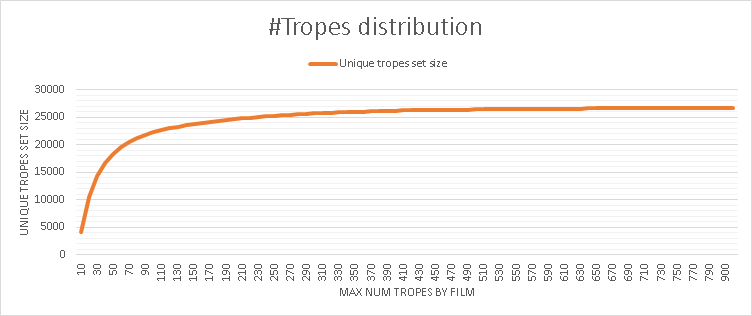
\includegraphics[width=0.9\linewidth]{../images/tropes_distribution_chart.png}
		\caption{Accumulative distribution of tropes dassociated to films}
		\label{fig:tropesdistributionasociatedtofilms}
	\end{figure}
	 
	The challenge now is how to create a corpus that will be usefull to find relationships between tropes and films. Each film have a description and a list of tropes, and each trope have a description and a list of films that uses this trope. Initially our dataset obtained from tvtropes.org 13th december 2019 included 12360 films and 26742 different tropes (25405 after remove duplicates). The film with higher number of tropes has 1028 tropes and the film with minimum number of tropes has 0 tropes. Tvtropes dataset has 673258 pairs film-trope. 73917 duplicate values in pairs. After apply word2vect to artificially created corpus, a set of embeedings vectors will be created. The embeeding vector integrate information about the context of a certain word and it is easy to find the relationships with other terms in corpus.\\
	
    The size of the corpus of variations without repetition of 15 tropes taken from 9 in 9 is 288Mbytes. 9-size phrases have been created by making variations without repetition and ordering the result randomly \\
	
	\begin{center}

${v}_{m,n} = m.(m-1).(m-2)...(m-n+1)$
${v}_{15,9} = 1816214400$
	
    \end{center}
	
	Below first lines of corpus generated file:\\
	\texttt{    
	ChuckCunninghamSyndrome AccidentalMisnaming EpicFail CassandraTruth BeeAfraid AgonyOfTheFeet Fainting BandageMummy Fingore. EpicFail AccidentalMisnaming CassandraTruth BandageMummy BeeAfraid ChuckCunninghamSyndrome Fainting AgonyOfTheFeet Invisibility. PopTheTires EpicFail Fainting BandageMummy AccidentalMisnaming AgonyOfTheFeet ChuckCunninghamSyndrome CassandraTruth BeeAfraid. AccidentalMisnaming ScreamsLikeALittleGirl AgonyOfTheFeet CassandraTruth BeeAfraid Fainting ChuckCunninghamSyndrome EpicFail BandageMummy.}\\

%       % This kind of thing does not belong in a paper 
%     Following line represent word2vec train parameters:\\
% \begin{verbatim}
% /word2vec 
% -train ngrams_15_taken_9.txt 
% -output ngrams_15_taken_9.bin 
% -cbow 1 -size 200 -window 8 
% -negative 25 -hs 0 
% -sample 1e-4 -threads 20 
% -binary 1 -iter 15
% \end{verbatim}

% There's no need to say what to do; focus on the results and the
% methodology. Mechanical steps can be explained in the repository.
      
	\begin{figure}
		\centering
		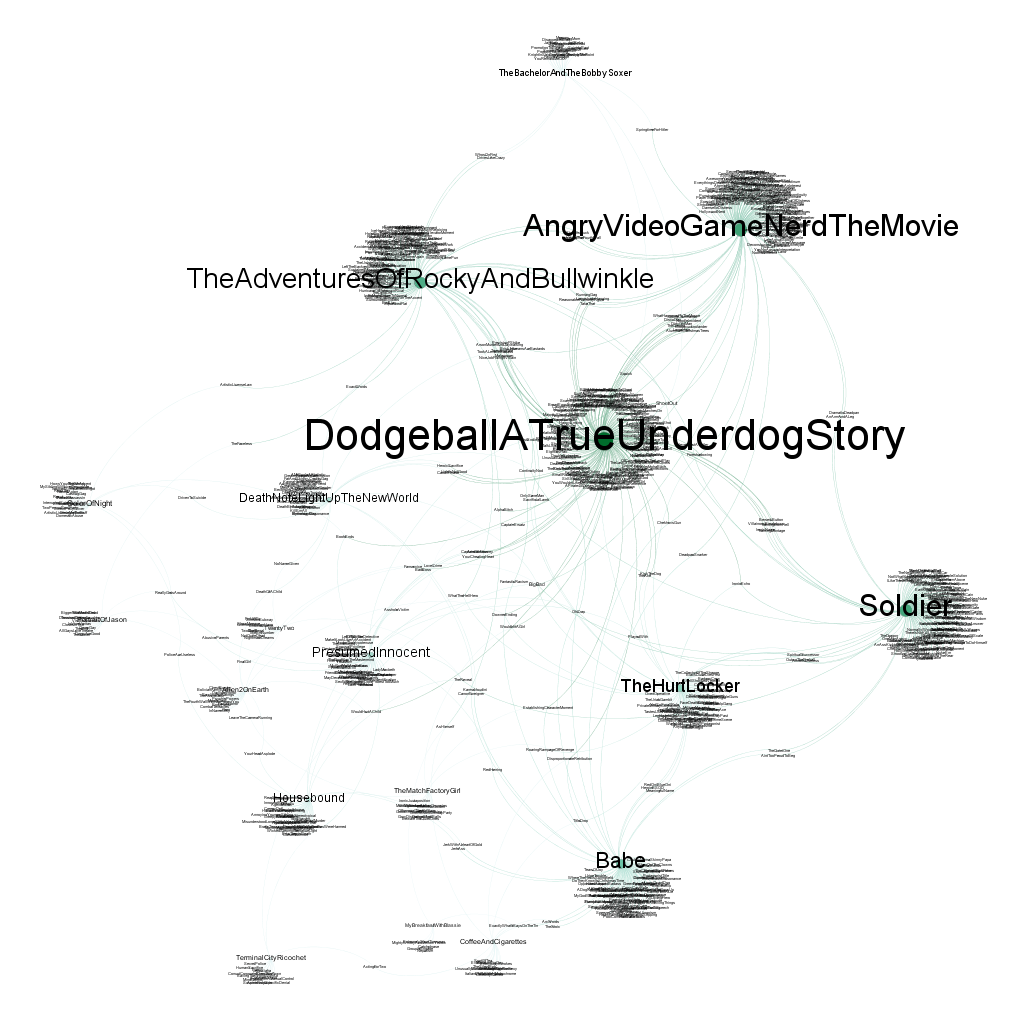
\includegraphics[width=0.9\linewidth]{../data/gephi/pairs_films-trope_1k_v3}
		\caption{}
		\label{fig:pairsfilms-trope1kv3}
	\end{figure}

	4. Build word2vec model. After that we will have a numerical vector for each trope. \\
	5. Visualize tropes vector space in order to detect clusters and possible data organization. \\ 
	6. Create a Vector for each film as the sumatory of all tropes vectors. \\

        \section{Results}
        \label{sec:res}
        
        \section{Conclusions, discussion and future work}
        
	\section{Acknowledgments}
	
	\bibliographystyle{iccc}
	\bibliography{iccc}
	
\end{document}
